\begin{figure}[h]
	\centering
	\label{fig:distribution}
	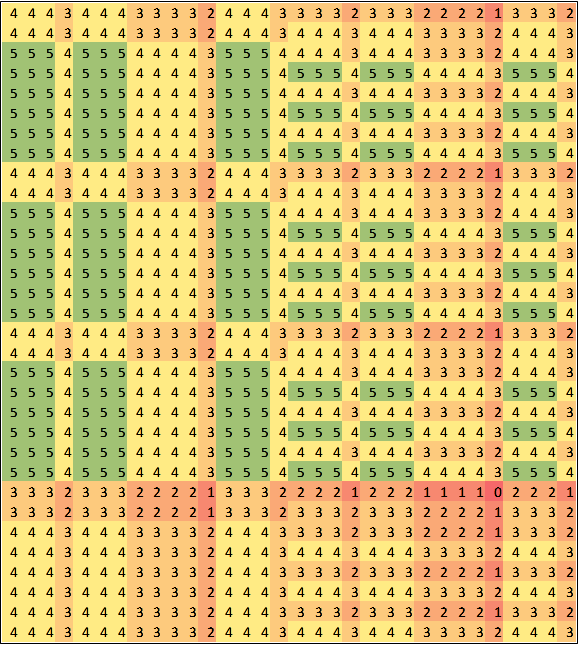
\includegraphics[width=2.5in]{contents/00_images/D(tacgt)}
	\caption{
		Distribution $\mathcal{D}$(\texttt{tacgt}) of Hamming distances from \texttt{tacgt} \cite{sia2015}
		to all $4^{5} = 32\times32$ $k$-suffixes of length 5.
		The value in the $p^{th}$ cell of this $32\times32$ table (at row $\frac{p}{32}$, col $p$ \emph{mod} 32) is the Hamming distance from the \textbf{center} \texttt{tacgt} to the $k$-suffix that maps to the binary number $p$.\newline
		%, i.e. $D(z)_{p} = dH(z,\emph{unmap}(p))$.\newline
		Ex. $\mathcal{D}(\texttt{tacgt})_{100} = dH(\texttt{tacgt}, \texttt{acgca}) = 5$.\newline
		%$D(\texttt{tacgt})_{24,27} = dH(\texttt{tacgt}, \emph{unmap}(795)) = dH(\texttt{tacgt}, \texttt{tacgt}) = 0$.
	}
\end{figure} 